\chapter{Notation Metamodel}
In order to bridge the gap between a model and a token stream a notation model is developed. The notation model is an EMF model, so it is possible to persist the notation model seperatly from the language model. The existence of a notation model in general after a token stream or a language model is created is optional with one exception. The exception is the use of morphems without default or language element representations. Due to this fact, they should be avoided. It is possible to create a notation model from a word of a language or from a model which complies to the additional constraints introduced by a grammar. The presented notation model does not include additional layout information, like in most cases newlines, spaces, tabs or for visual editors coordiantes, styles, etc. In gereral, the notation model saves information which is not stored in the language model but relevant for presentation.\\

The main purpose of the notation model is to unambigiously describe a word which produces the language model and to enable to chooce different representations for grammar parts by providing hints for the unparser.

The main design considerations for development of the notation metamodel are:
\begin{itemize}
	\item to be able to fully represent and subsitute a parse tree, so pretty printing could be done easily.
	\item to support the creation of the parse tree from an AST. This means that it must be possible to guide the unparsing process by hints and hold alternative choices to choose. To be able to distinguish alternative productions requires granularity up to parse tree level.
	\item to have one notation element container per \code{EObject}. This does not not only eases reasoning, but also allows stable paths if the corresponding notation element is a generic container. With the use of an \code{ECrossReferenceAdapter} for the refered language models resource, it is possible to obtain the corresponding notation element even if the structure of the notation model is lost. 
\end{itemize}

A notation model will refer grammar elements, so before the notation metamodel can be developed, an EBNF grammar metamodel will be defined. \\

As convention, transient model elements are modeled as private static elements with a leading \code{-} and underlined.

\section{Grammar Metamodel}
%%%%%%%% GrammarMM	%%%%%%%%%%%%%%%%%%%%%%%%%%%%%%
\begin{figure}
\centering
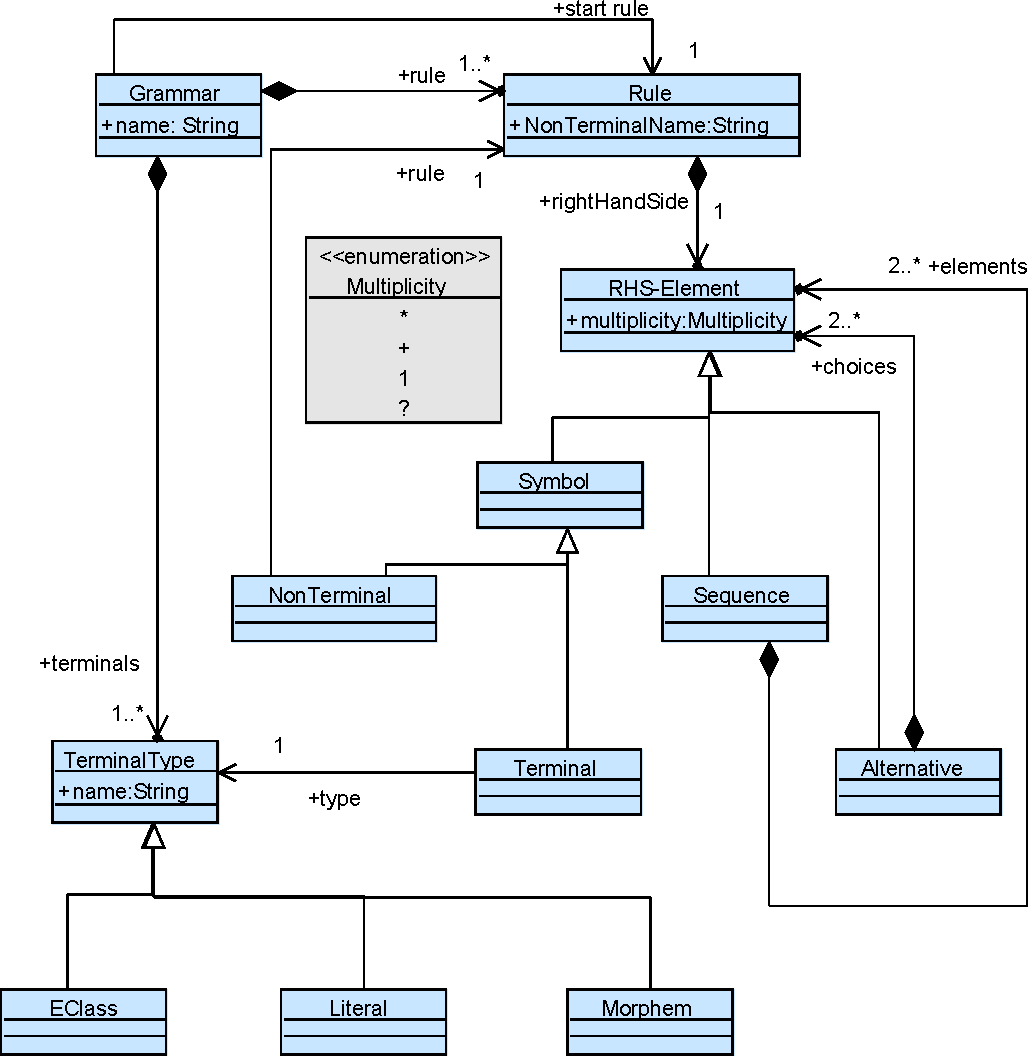
\includegraphics[scale=0.85]{gfx/ex/Grammar_CFG} 
\caption{EBNF Grammar Metamodel}
\label{MM:EBNF}
\end{figure}

Figure \ref{MM:EBNF} shows a metamodel for an EBNF grammar. The metamodel lacks the ability to define lexemes  \\
Compared to the definition of a CFG, the non terminals are the set of \code{NonTerminalName}s of \code{Rule}, the terminals are the set of \code{name}s of \code{TerminalType}, the start symbol is the \code{Rule} refered by \code{Grammar} and the productions are implicit described by the directly and indirectly contained elements of the \code{Rule}s. The \code{NonTerminal} and \code{Terminal} elements in the grammar are just refences to the real non terminals and terminals. This definition overlap is owed to the fact that the same terminal may appear multiple times in productions, which must be distinguishable . This denomination allows for example in following rule
\\\begin{code}
A : b$_1$ C b$_2$
\end{code}\\
to be \code{b$_1$} an instance of \code{Terminal}, \code{C} and instance of \code{NonTerminal} and \code{b$_2$} another instance of \code{Terminal}, but refering to the same \code{TerminalType}.

The \code{Grammar} has at least one \code{Rule} and one \code{TerminalType}. The \code{Grammar} has exactly one \code{start rule}. The \code{Rule}s have a name and contain exactly one element as their \code{rightHandSide}. This element might be either a \code{NonTerminal}, a \code{Terminal}, a \code{Sequence} or an \code{Alternative}. \code{Sequence}s and \code{Alternative}s are containers for at least two \code{RHS-Element}s. \code{Sequence} are \code{a b c} or \code{(a b)+} for example. \code{Terminal} and \code{NonTerminal} hold references to their unique type they represent. \code{Symbol} just provides abstraction but does not add expressivity to the language itself. Every \code{RHS-Element} has a \code{Multiplicity}, so exactly one \code{1}, one or none \code{?}, zero or more \code{+} or any mutltiplicity \code{*} can be expressed. Subclasses of \code{TerminalType} are present to allow a more detailed specification of \code{TerminalType} in later models.


%%%%%% GrammarMM()	%%%%%%%%%%%%%%%%%%%%%%%%%%%%%%

%% Grammar Instance
\section{Grammar Example}
\begin{figure}
\centering
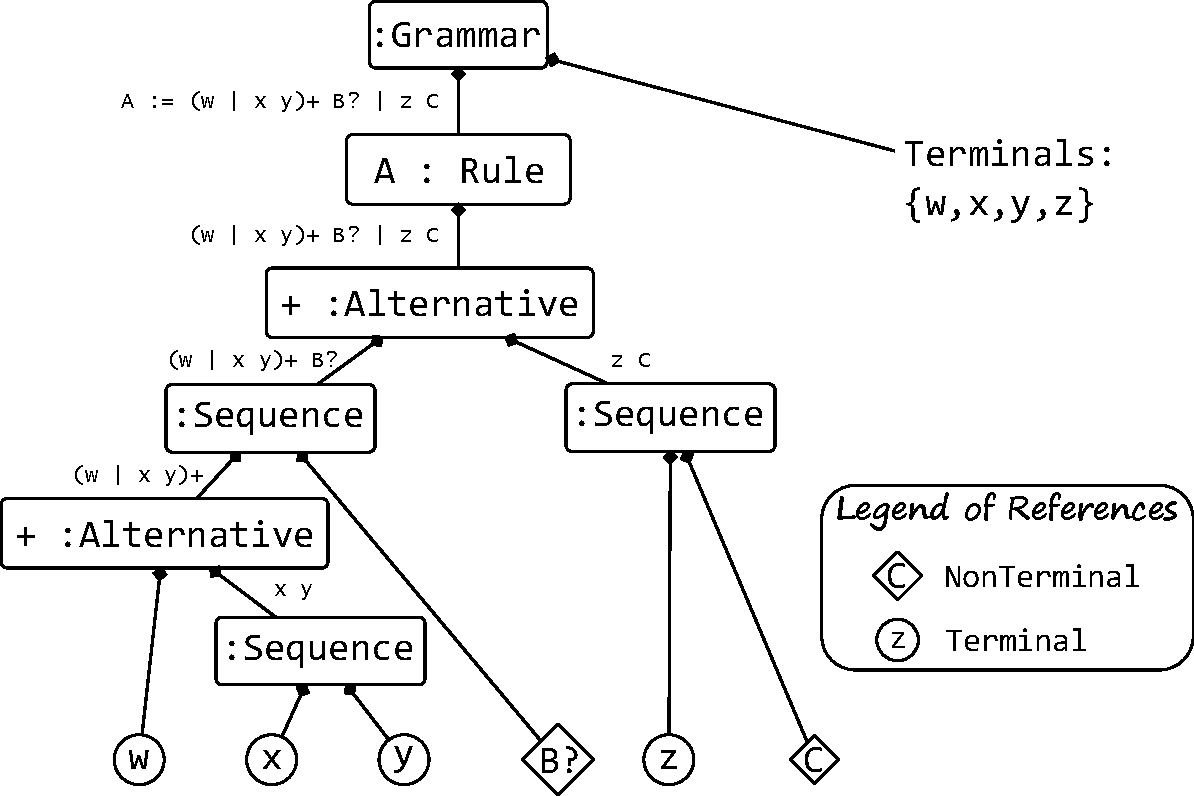
\includegraphics[scale=0.7]{gfx/ex/grammarExample} 
\caption{Example Rule ``A := (w |x y)+ B? | z C''}
\label{MM:GrammarExample}
\end{figure}
Figure \ref{MM:GrammarExample} shows the model instance of the EBNF metamodel \ref{MM:EBNF} of the grammar  \code{A := (w |x y)+ B? | z C}. The grammar rules \code{B} and \code{C} are left out, as well as the start rule reference. The references to the symbols \code{w}, \code{x}, \code{y} and \code{z} are replaced with the name of the referenced symbol.

\section{Attributed Grammar}
\begin{figure}
\centering
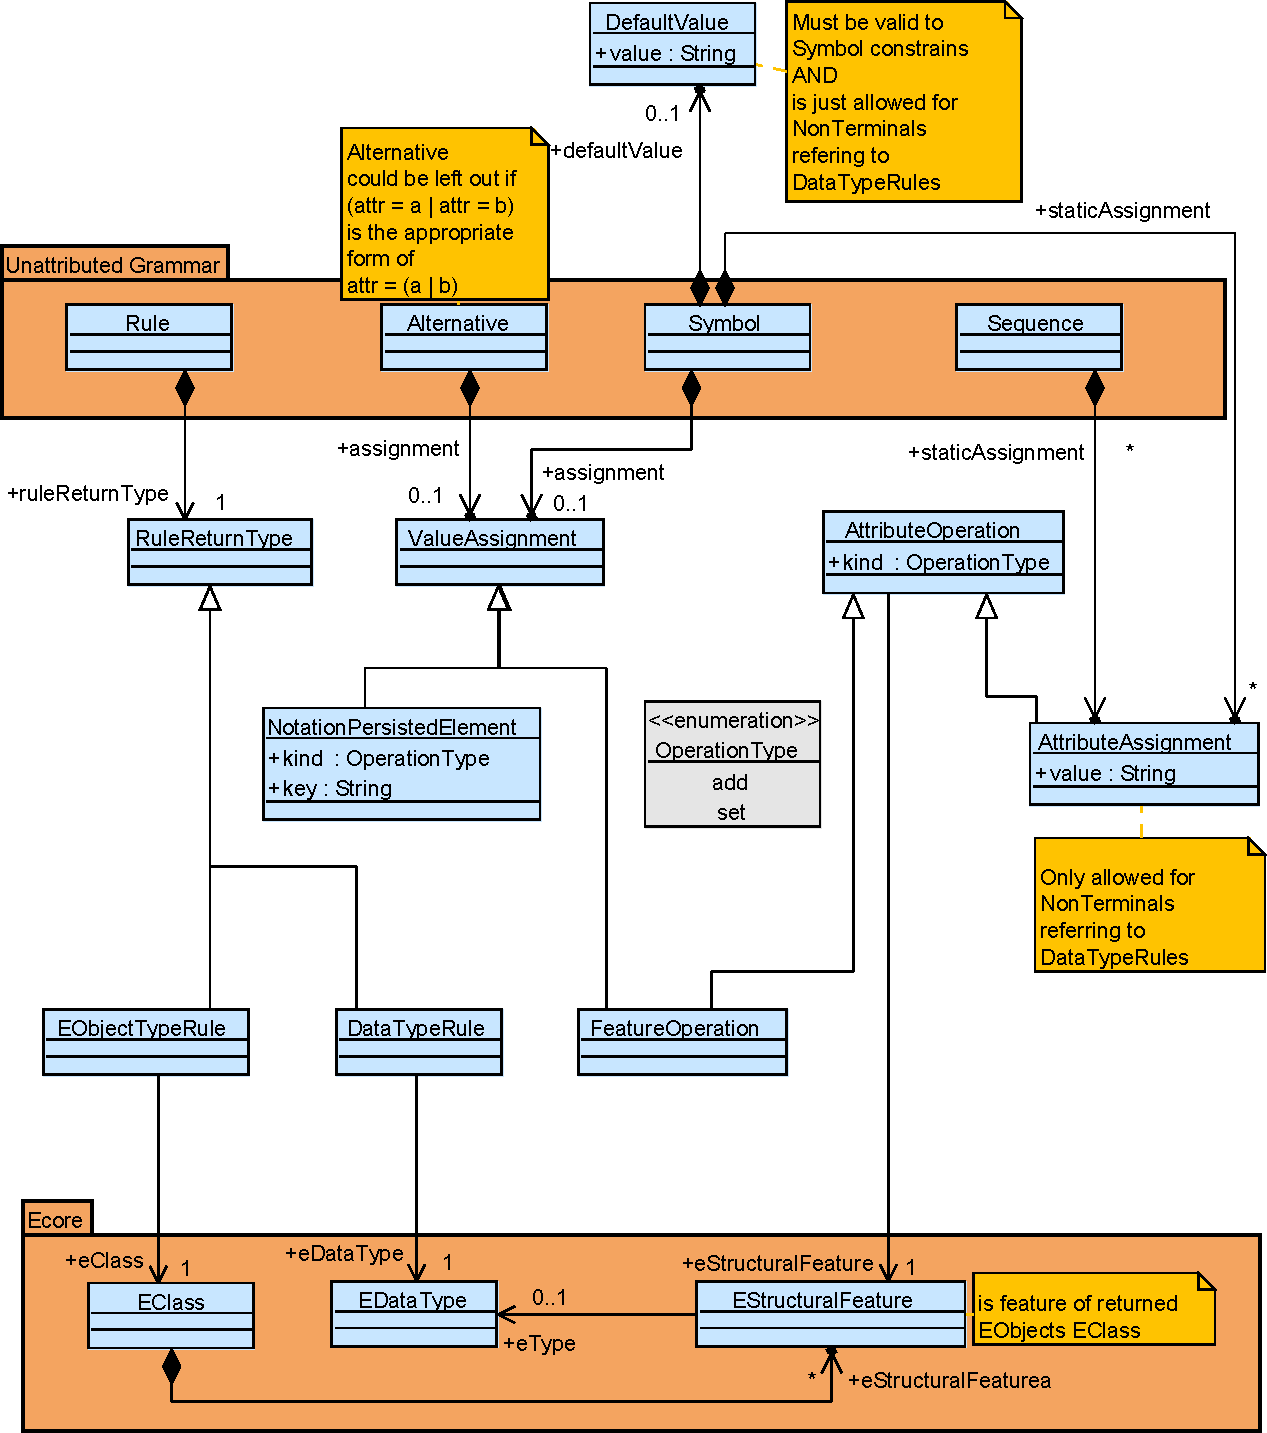
\includegraphics[scale=0.7]{gfx/ex/Grammar_Attributed} 
\caption{Attributed Grammar metamodel extension}
\label{MM:AEBNF}
\end{figure}

The metamodel defined in \ref{MM:AEBNF} adds attributation and default values to the grammar. It uses metaclasses from the metamodel \ref{MM:EBNF} for CFGs. The packaging is for documentation purpose only, because the metaclasses of the CFG metamodel refer to the current metaclasses. \\
Each \code{Rule} has a \code{RuleReturnType}, which might be an \code{EClass}, if it is a an \code{EObject} returning rule or an \code{EDataType}, if it is a Data Type Rule. The addionaly distinction in \code{EObjectTypeRule} and \code{DataTypeRule} is for presentation purposes only, this makes it obvious in the diagram when an \code{EObjectTypeRule} is used. For a real implementation a reference from \code{Rule} to an \code{EClassifier} would be sufficient. \code{EClassifier} is the supertype of \code{EClass} and \code{EDataType}. \code{Symbol} now can contain a  \code{defaultValue}, which is a \code{String}.  \code{String}s are structureless, so the use of \code{DefaultValue}s is restricted to  \code{NonTerminal}s refering \code{DataTypeRule}s and  \code{Terminal}s only. The  \code{String} must not violate the  \code{Symbol}s constraints. Given the example \code{attribute+=TerminalSymbol}, an attribute assignment is realized by \code{TerminalSymbol} containing a  \code{FeatureOperation} with \code{kind} set to  \code{add} and a reference to the  \code{EStructuralFeature} named \code{attribute}. The \code{EStructuralFeature} must be contained in the  \code{EClass} of the returned \code{EObject}s type. In contrast to Xtext, it is possible to assign statically a structureless value to an attribute, for example 
\begin{xtxt}
Rule : {ruleAttribute="true"} "1"
\end{xtxt}   
which means that if the rule matches \code{ruleAttribute} is assigned to \code{"true"}. This can be done for an abitrary amount of \code{EStructuralFeatures}. \code{NotationPersistedElement} allows to persist a String in the notation model, this allows to share data between \code{Alternatives}. \\
\code{Alternatives} also contain a \code{ValueAssignment}. This could be omitted if 
\begin{xtxt}
attribute= (a | B)
\end{xtxt}
would not be allowed and instead only the alternative 
\begin{xtxt}
(attribute = a | attribute = B)
\end{xtxt}
would be allowed.
%% Grammar Instance()

\section{Notation Metamodel}
%% Prod
\begin{figure}
\centering
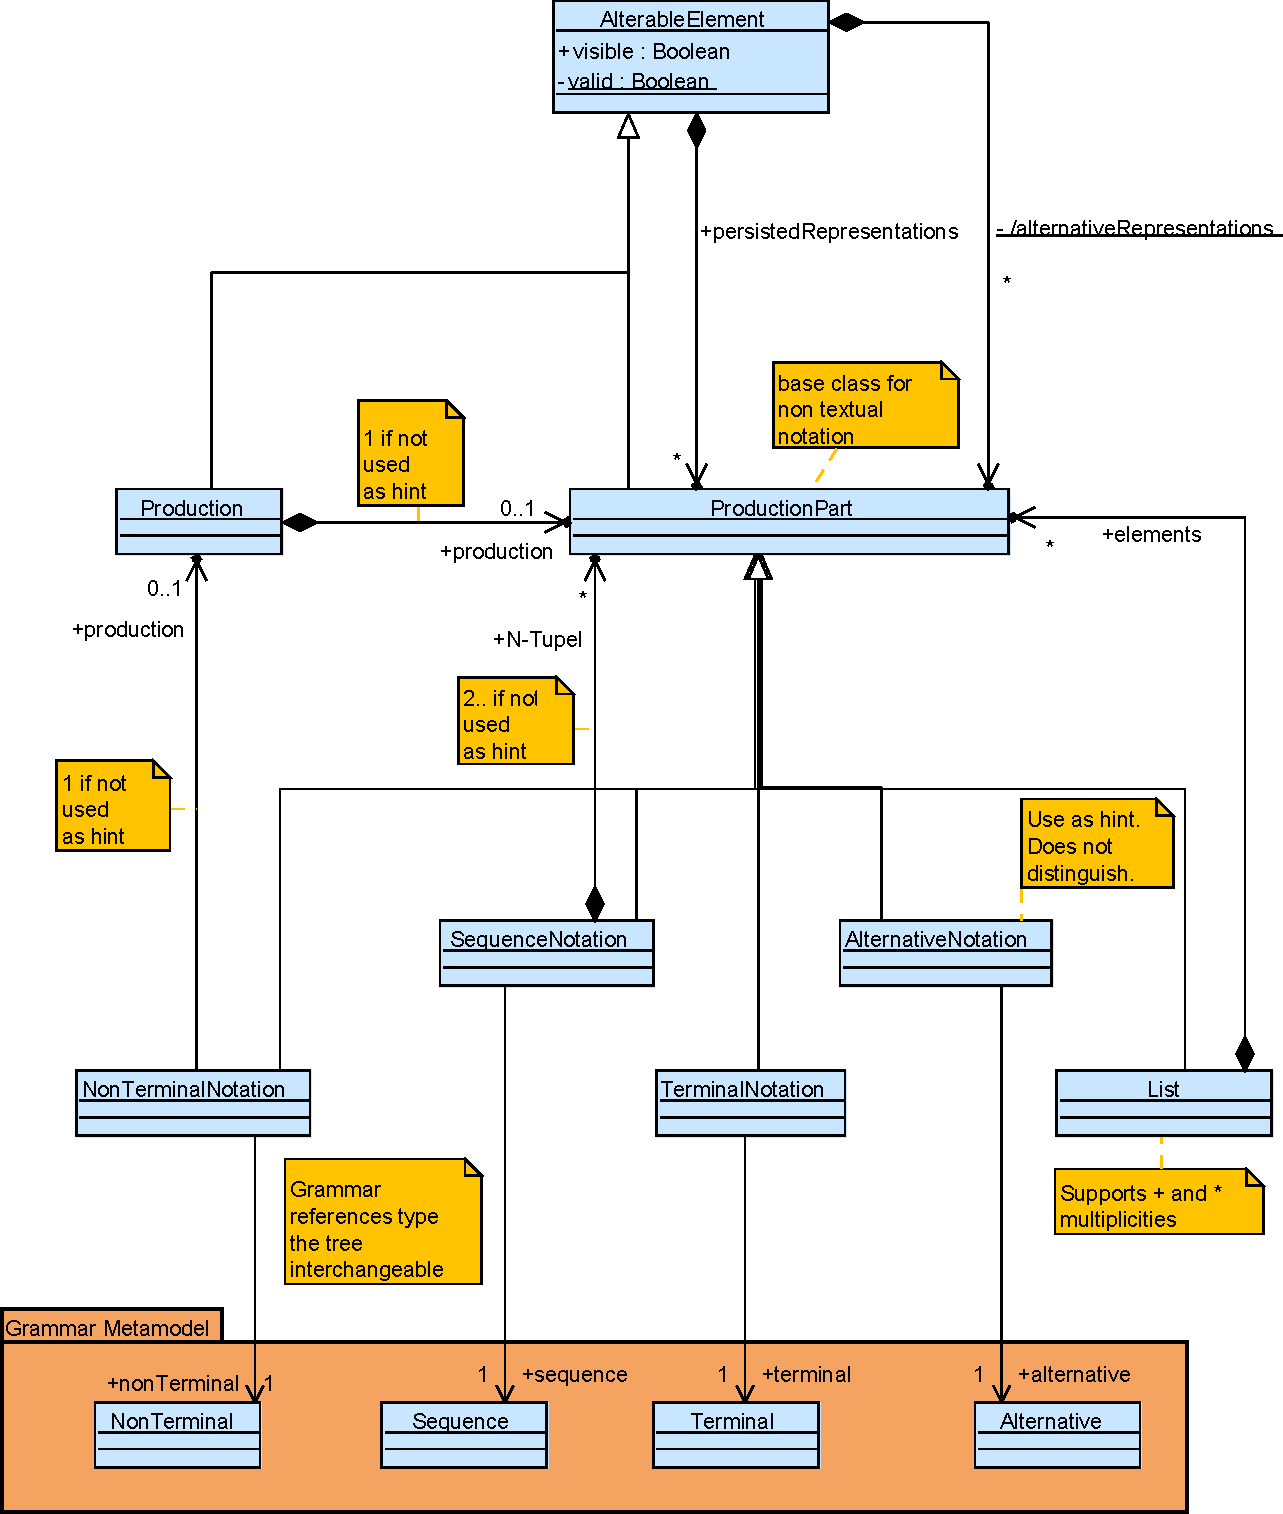
\includegraphics[scale=0.65]{gfx/ex/Notation_Prod} 
\caption{Production part of Notation metamodel}
\label{MM:Not:Prod}
\end{figure}

The diagram \ref{MM:Not:Prod} shows the section of the notation metamodel which is relevant for its function representing a parse tree and guiding unparsing. It is able to represent parse trees up to terminals, but does not contain the token values.\\

\subsection{Evolving from a simple parse tree metamodel}The metamodel in diagram \ref{MM:Not:PT} is sufficient to describe a parse tree, where \code{TerminalNotation}s represent the leafs and \code{NonTerminalNotation} the branches. It contains a subset of elements of the notation model, namely \code{NonTerminalNotation}, \code{TerminalNotation} and \code{ProductionPart}. The relationship of the subset elements differs from \ref{MM:Not:Prod} in that \code{NonTerminalNotation} contains \code{ProductionParts} direcly, but more importantly also that \code{NonTerminalNotation} can contain multiple \code{ProductionPart}s. \code{NonTerminalNotation} and \code{TerminalNotation} are of a generic type, to determine which Symbol they represent, they refer to \code{NonTerminal} and \code{Terminal}. The distance to the symbol is one, the distance to the symbol type is two. 
For example, in the following grammar, the type of the \code{b}s are equal, but the \code{b}s are not:\\
\code{S : b c | b d} \\
A verbose representation of this grammar would be: \\
\code{S : b$_1$ c | b$_2$ d} \\
\code{TerminalNotation}s refer to the exact position in the grammar, in the previous example for example to \code{b$_1$} and the position in refers to the type \code{b}. For an concrete parser implementation, this means that in case of a shift reduce parser, the reference to the \code{NonTerminal} can be at least one production later as normal, because the type is known when the rule is reduced but the position is not known until its producing production is reduced. The exact positions is useful to guide unparsing and the referecing solution provides flexibility while keeping stable \code{NonTerminalNotation}s and \code{TerminalNotatation}s. The parse trees is created by this metamodel need post processing to group make their structure. For example acessing the last \code{b} in the tree created for the grammar:\\
\begin{xtxt}
A : b+ c b 
\end{xtxt}
with the input \code{b b b c b} requires to iterate over each element. 

\begin{figure}
\centering
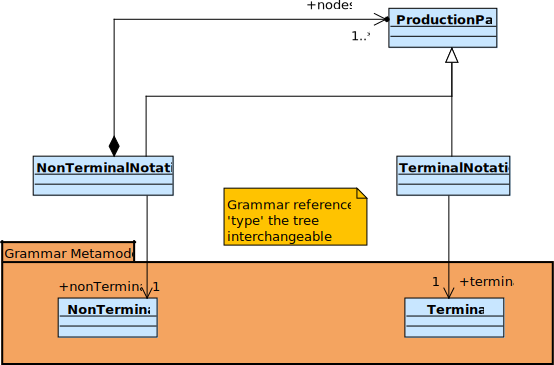
\includegraphics[scale=0.75]{gfx/ex/Notation_ParseTree} 
\caption{Simple parse tree metamodel}
\label{MM:Not:PT}
\end{figure}

\subsection{Term parse tree metamodel}A metamodel able to hold terms structured is shown in \ref{MM:Not:TT}. The \code{NonTerminalNotation} holds exactly one reference to a \code{ProductionPart} named \code{production}. The distinction in different terms is held by \code{SequenceNotation} which contains an \code{n-tupel} of at least two \code{ProductionParts}. A \code{List} holds \code{Symbol}s with a possible multiplicity higher than one. It might be benefical to directly support multiple values per \code{ProductionPart}, for example \code{a+}, but this would not render \code{List} obsolete in order to support \code{(a | B)+}. Since alternatives do not occur in a parse tree, because one choice must have been used, they have no equivalent in a parse tree. 

\begin{figure}
\centering
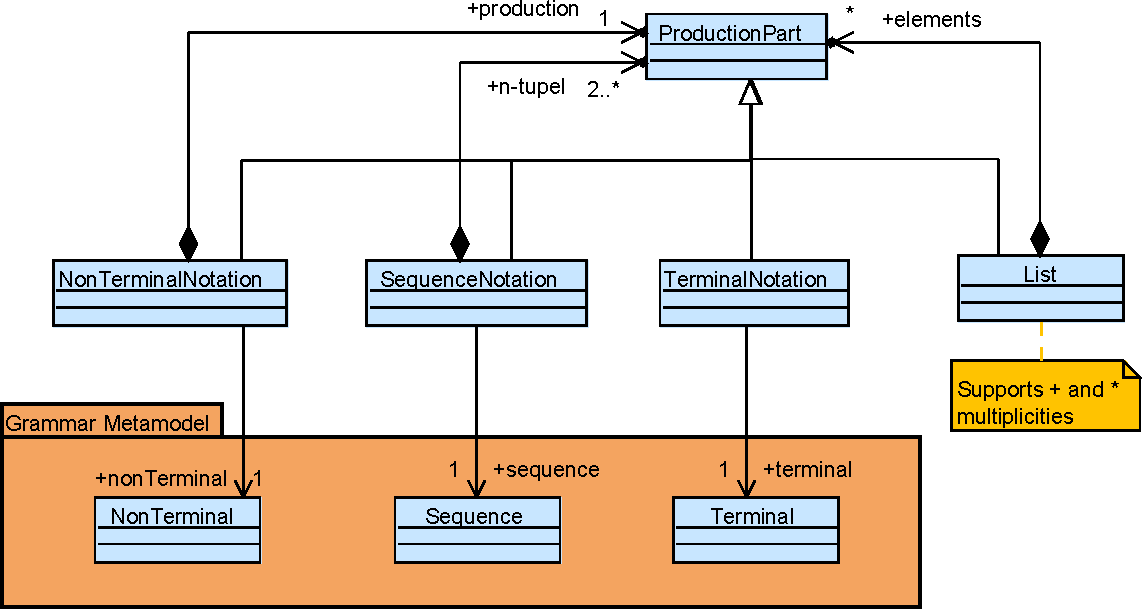
\includegraphics[scale=0.75]{gfx/ex/Notation_TermTree} 
\caption{Term parse tree metamodel}
\label{MM:Not:TT}
\end{figure}

\subsection{Production part of the Notation model}
Figure \ref{MM:Not:Prod} shows the final production part of the notation metamodel. It differs from the one used for terms in following points:
\begin{itemize}
	\item an additional indirection from \code{NonTerminalNotation} to \code{ProductionPart} was introduced. 
	\item \code{AlternativeNotation} to represent \code{Alternative}s was added.
	\item The multiplicites of the references are less constrained regarding the lower bound.
	\item \code{AlterableElement} was added.
\end{itemize}
The use of the additional indirection from \code{NonTerminalNotation} to \code{ProductionPart} via \code{Production} decouples the \code{Production}. The reason for this is the use of \code{Production} as the complementing element for a language element. This is described in more detail in \todo{ref} and is one of the main design targets of the notation model.\\
As stated in \todo{ref} \code{AlternativeNotation} is not needed to represent a parse tree. It is the only \code{ProductionPart} which does not contain and does not refer to data or another \code{ProductionPart}. \code{TerminalNotation}s link to data is described in the seperate diagram \ref{MM:Not:DataLink}. \code{AlternativeNotation}s only use is to hint while unparsing. For example, without \code{ProductionPart} for the given rule
\begin{xtxt}
R : ((a | b) | (c d)) 
\end{xtxt}
it is possible to hint to each element individually, but it would be impossible to hint to the alternative \code{(a | b)}. \\
To be able to hint to a specific grammar element without requiring a representation is the reason the lower bounds of all references have been removed. This must be possible during unparsing.\\
\code{AlterableElement} is the base class of all production related classes. Its main task is to hold \code{alternativeRepresentations} for itself. These \code{alternativeRepresentations} are not persisted and are derived by the unparser or in other words set by the unparser. \code{AlterableElements} also contains a set of \code{persistedRepresentations} maintain former representations, for example. These do not need to be a subset of the current \code{alternativeRepresentations}. Its dedicated use is to restore former representations, which are or became again valid.

\section{Production part of the Notation model} \label{sec:MM:Not:Prod}
Figure \ref{MM:Not:LR} shows how the connection of the Notation metamodel to the language model is made. The two central metaclasses in this diagram are \code{EObjectProduction} and \code{LanguageTokenContent}. The root of the notation model is \code{NotationModelRoot}. It contains the \code{rootProduction} of the parse tree. This might be an \code{UnassignedRuleProduction}, but in general an \code{EObjectProduction}. The connection between both are is established by the reference \code{languageElement} of \code{EObjectProduction}.  The type of the refered instance must be the refered type of the \code{EObjectTypeRule} at \code{type} reference of \code{EObjectProduction}. \code{EObjectProduction}s are the only notation elements which establish a direct connection between the notation model and the language model. \code{EObject}s, like Java objects, are the only refereable instance at runtime. Thus, a structurally identical containment relationship based tree with language objects on the one and \code{EObjectProduction}s on the other side is created. The subtrees of an notation node, \code{EObjectProduction} are stored in its \code{children} containment. This complements the vanished containment relation between \code{NonTerminalNotation} and \code{Production} in figure \ref{MM:Not:PT}. This design allows each \code{EObject} production to contain its own part of the parse tree, integrating parse tree and structually symetric language tree on a per \code{NonTerminalNotation} base. \code{NonTerminal}s are the only part in the grammar where \code{EObject}s are produced, but \code{NonTerminal}s may also produce \code{EDataType}s or refer to a rule which is an unassigned rule call. To store productions in the parse tree where no \code{EObject} is produced, \code{NonTerminalNotation} contains a derived \code{nonEObjectProduction} containtment. This containment is derived, because it is just set in the case where \code{production} is not of type \code{EObjectProduction}. This reestablishes the missing containment reference in the case where the \code{Production} is not contained by the \code{EObjectProduction} tree. \\
The other notation class which needs to establish a connection to the language elements is \code{LanuageTokenContent}. \code{TokenContentAdapter} are responsible to fill in the token value while the token stream is created during pretty printing of the parse tree. This is explained in \todo{ref}. \code{LanuageTokenContent} is responsible to assign the token content based on a value of an instance of an \code{EStructrualFeature} of an \code{EObject} in the language model. Because instances of \code{EStruturalFeature}s are not referable, \code{LanguageTokenContent} uses a reference to the \code{EObject} and reflection to obtain the value of the \code{EStructuralFeature} instance defined by the \code{eStructuralFeature} reference of \code{FeatureOperation} of the attributed grammar metamodel. The reference to the necessary language \code{EObject} is obtained by the first parent \code{EObjectProduction} in the notation models containment hierarchy. The \code{index} of \code{LanuageTokenContent} determines the exact value of an \code{eStructuralFeature} in case of an multiplicity higher than one, for example if an \code{EAttribute} is of type of multiple (list of) strings.

%% Prod
\begin{figure}
\centering
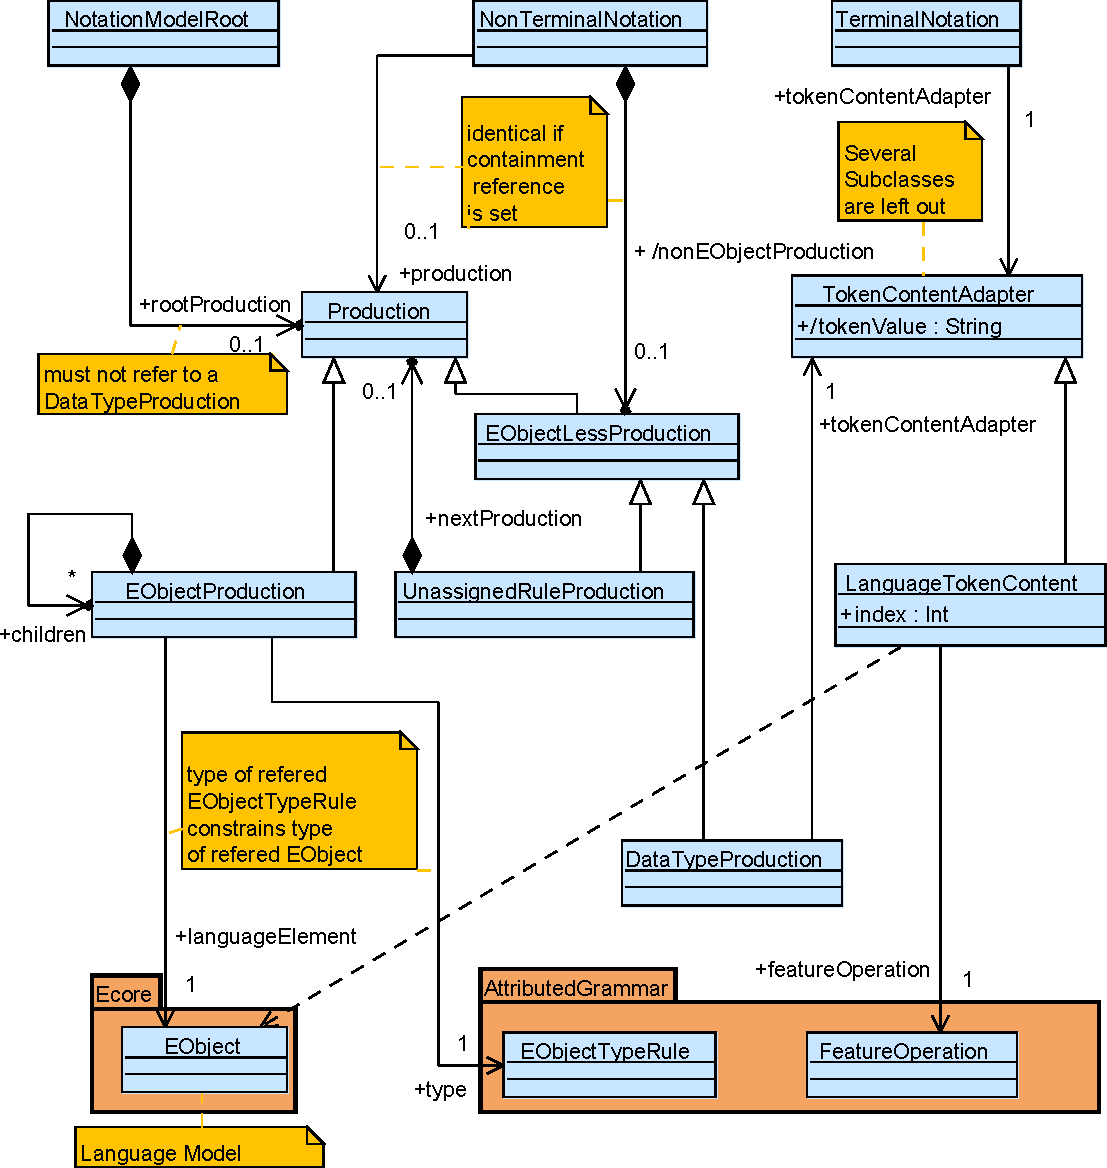
\includegraphics[scale=0.8]{gfx/ex/Notation_LangRel} 
\caption{Language model connection}
\label{MM:Not:LR}
\end{figure}

\section{Token value connection}
Diagram \ref{MM:Not:DataLink} shows the relation of notation elements to the token value. Except for the \code{token} reference of \code{TokenContentAdapter}, this is only relevant for pretty printing of the parse tree. The abstract \code{TokenContentAdapter} is the central class in the diagram. Each \code{TerminalNotation} and each \code{DataTypeProduction} refers to exactly one. Because both hold the content of a structureless value, this unifies both in regard to pretty printing. \code{TokenContentAdapter} has a derived attribute named \code{tokenValue} of type string. The value of \code{tokenValue} is determined by the use of \code{ValueConverter}s, in order to convert between an non character type, for example \code{EInteger} and the only valid output value of Tokens, characters. The use of the transient optional reference to \code{Token} is twofold, first it enables the Notation model to hold references to both, the content of a \code{Token} on the token stream and its content in the language model, thus optionally keeping both synchronized. Second this existance is mandatory to hold the textual representation of cross references until they are resolved to an URI or completely. Subclasses of \code{TokenContentAdapter} represent the different possibilites of data sources for the token content:
\begin{itemize}
	\item \code{LanguageTokenContent} is explained in \ref{sec:MM:Not:Prod}.
	\item \code{GrammarTokenContent} the value of the token depends on a \code{Literal} \code{value} defined in the grammar metamodel.
	\item \code{NotationTokenContent} the value of the token is contained by an \code{NotationPropoerty} in the notation model. The key is obtained by a reference to an instance of \code{NotationPersistedElement} from the  attributed grammar metamodel.
	\item \code{MagicTokenContent} is used when the data source is none of above. It is used if the content is set programtically.
\end{itemize}


\begin{figure}
\centering
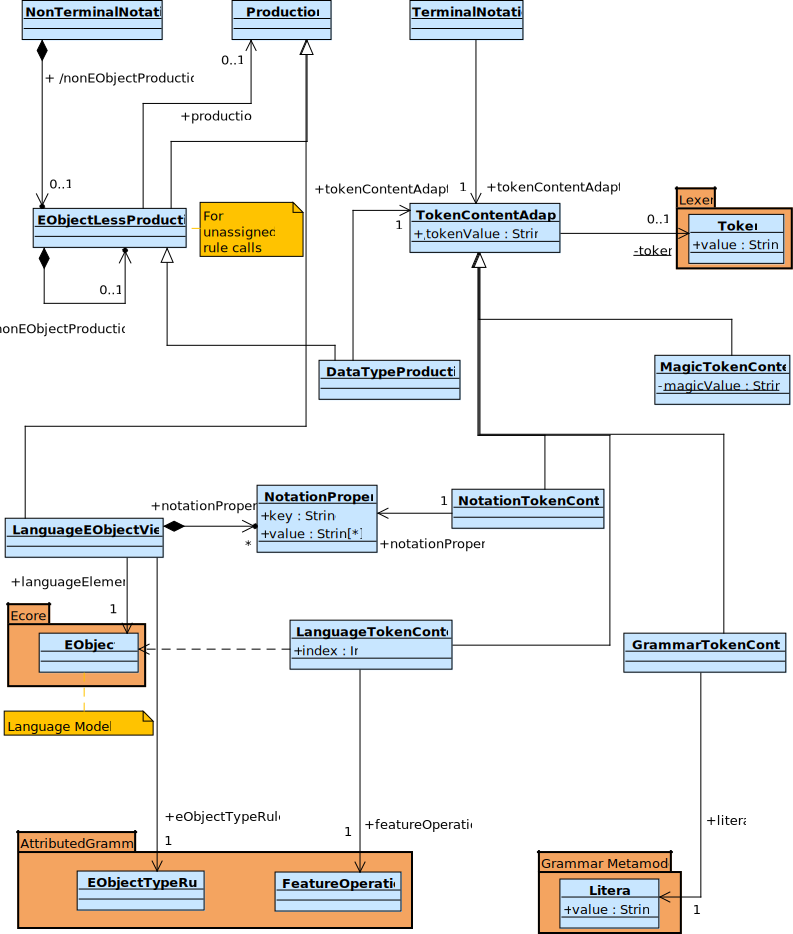
\includegraphics[scale=0.7]{gfx/ex/Notation_DataLink} 
\caption{Token value connection}
\label{MM:Not:DataLink}
\end{figure}

\section{Compression of the notation model}
To create a token stream it is necessary to create the complete parse tree structure in the notation model. This structure is more verbose than what is necessary to uniquely identify a word. Due to the fact, that the notation model serves as a building plan to create a word, it is just necessary to persist the part of the notation model which eleminates all ambiguities. For example, for the following rule:
\begin{xtxt}
A:  "keyword1" v=ID 
 |  "keyword2" v=ID
\end{xtxt}
it is just necessary to store which rule was chosen, for example the one containing \code{"keyword1"}, but not the expanded parse tree. It unparsing is predictable, it is even possible to omit this distinction if the selected option is equals the default option of the unparser.  \\
It is furthermore possible to enumeration the alternatives and save their values instead of the references to the \code{ProductionPart}s.

\section{Conclusion}
The unparser combined with the notation model allows to choose different textual respresentations for a language model. 



\chapter{Combining Stuff}
\section{Notation MM as Sentential tokens}
\section{Notation MM as graphical editor base}
\section{Conclude graphical editor integrated in the grammar at Symbol, Seq, or Alt positions}
\section{what misses? Text <-> Model sync}





\subsection{Introduction}
Requirements:
\begin{itemize}
	\item In contrast to Xtexts node model which is just updated during parsing and used to guide unparsing, the Notation metamodel must be equivalent to a valid token stream and therefore describe it unambigiously. 
	\item It must contain or refer to all information to nesessary to create a specific token stream together with a language model and a grammar model.   
	\item it has to be a parsetree in order to create language elements if the correspoding tokens exist.
	\item it should offer GMF stuff elements \todo{add what GMF has interesting}
	explicit, seperated from language model
\end{itemize}




\section{old ==>}
%	-------------- Latex testing --------------
The Notation model is an EMF model to describe a tree. A node or leaf contains a reference to the describing language model element.The notation model bridges the token stream and the abstract syntax. It is the parse tree, and thus also describes a valid concrete syntax representation of the model.  It is a mandatory to updated or created it when generating a concrete representation of the model. If the notation model (element) was created to complement a language model (element), the notation model (element) serves as a disambiguis bulding plan to create the token stream for a valid concrete representation. In gereral, the notation model saves information which is not stored in the language model but relevant for presentation. It also keeps a generic, type save reference on the represented language object.\\
Each notation element represents (part of) a language element and should be a stable container for different visual representations of that element with addionaly layout information.  Due to this, if an element has multiple semantically equivalent representations, it is possible to switch the representation without switching the notation element. A switch would invalidade the descendants of the current node. A notion element therefore contains a transient structural feature containing all possible valid concrete representation rules, the non-transient last representation rule and optional the last user selected representation rule. In case these representation rules are grammar rules, they must be complemented with addionional information in order to make the token production unambigious. For example a grammar rule like:
\begin{xtxt}
A : (B | C) "myKeyword"
\end{xtxt}
would be translated to the following productions rules 
\begin{xtxt}
A - > B "myKeyword"
A - > C "myKeyword"
\end{xtxt}
for the sake of abstraction and simplicity, this distinction, especially im more complex scenarios, should be hidden from the language developer. In a case where B and C are semantically equivalent  it is arbitrary from the abstract syntax perspective if an A contains a B or C. The notation element must close this gap, so an notation element refering to a lanuage element represented by A doesn't need to store the keyword "myKeyword", this information is implicit, but it must distinguish if the concrete presentation of this particular A should use B or C as a presentation selection. It is therefore not nessecary to explicity assign  a production rule but to implicity make one resolvable by dissolving the ambiguity for options and choices which have no representation in the language model. \\
The base class for representation rules must be general, or unspecific, enough allow non textual representations. Notation elements should prefer containment references instead of attributes to easy to ease merging, like the GMF notation model. In contrast to GMF, this driving motivation is not team support but easier automatic updating between old and new versions.\\
In order to integrate with incremental parsing, notation model elements should hold a transient integer which contains the distance to the first previous token accesing the current one in it's lookahead. \\
Finally, a notation model element should contain a flag if it is currently textually visible.
\todo{ rewrites possible}
\todo{ reason that a representation in text editor is necessary}
\todo{mention that addtionaly layout information can be added to a node}


